\section{Test di Valutazione}
\nocite{friedmanTest}
\nocite{wiki:Friedman}
Per poter analizzare i dati da un punto di vista statistico in modo da capire quale dei tre sistemi risulti essere migliore in un task di classificazione, è necessario utilizzare un test delle ipotesi che sia in grado di rigettare o confermare l'ipotesi nulla.

L'ipotesi nulla da rigettare in particolare sarà:
$$H_0 : \mu_{ALEPH} = \mu_{PROGOL} = \mu_{FOIL} $$
Mentre, l'ipotesi alternativa da accettare sarà:
$$H_1 : \mu_{ALEPH} \neq \mu_{PROGOL} \neq \mu_{FOIL} $$

Tra le diverse metriche calcolate per i diversi algoritmi, l'accuratezza è la metrica utilizzata affinché venga verificato il test delle ipotesi.

Poiché per ogni dataset è stata ripetuta la sperimentazione, il test delle ipotesi sarà condotto per ognuno dei cinque dataset separatamente.
Il test da effettuare dovrà rispettare i seguenti vincoli dettati dal dataset e dal tipo di sperimentazione che è stata effettuata:
\begin{itemize}
	\item \textbf{Numero di campioni maggiore di due}: Visto il quantitativo di campioni da analizzare, il test da scegliere dovrà essere in grado di processare un numero di campioni pari a tre.
	\item \textbf{Dimensione del campione limitata}: Dato che il valore dell'accuratezza è stato calcolato per ogni fold, la dimensione del campione sarà limitata a dieci, nonché il numero di fold creati. Questo fa si che il test da scegliere dovrà essere necessariamente un tipo di test non parametrico in quanto, visto l'esiguo quantitativo di elementi, non può essere garantita nè la omoschedasticità, nè che i gruppi dei dati appartengano ad una popolazione con distribuzione normale.
	\item \textbf{Campioni dipendenti}: a causa dell'utilizzo della tecnica della k-fold cross validation i sistemi sono stati analizzati utilizzando gli stessi identici fold, rendendo cosi dipendenti i campioni.
\end{itemize}

Visti i requisiti che il test dovrà rispettare, il test scelto per la verifica delle ipotesi è il Friedman test, il quale è un test non parametrico utilizzato per testare la differenza tra i diversi campioni correlati.
L'ipotesi nulla del test di Friedman è che non ci sia differenza significativa tra le variabili. Se la probabilità calcolata è bassa (P è inferiore al livello di significatività selezionato) l'ipotesi nulla verrà rigettata e si potrà concludere che almeno due delle variabili sono significativamente differenti con le altre.

Si è deciso di utilizzare un livello di significatività $\alpha$ pari al 5\%.

Per calcolare questo tipo di test è stato utilizzato un software atto a realizzare test statistici quale MedCalc \textcopyright.
Di seguito verrà mostrato un esempio di output restituito dal programma, in particolare, ciò che è stato restituito dal confronto tra i tre sistemi sul dataset MLJ discretizzato:
\begin{figure}[H]
	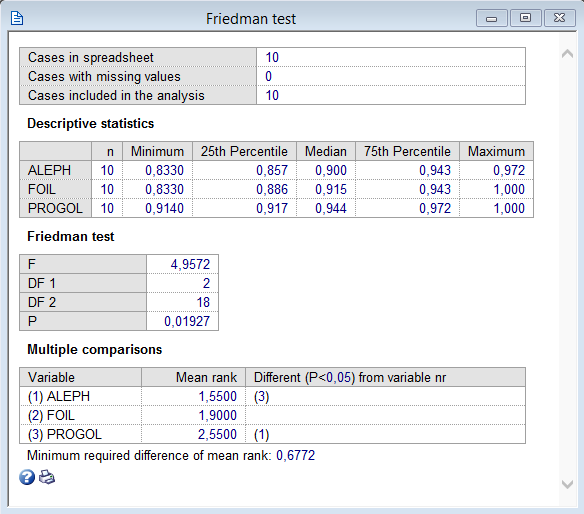
\includegraphics[width=0.9\textwidth]{img/TestResult/mljdiscr.png}
	\label{Friedman Test - MLJ Discretizzato}
\end{figure}

Riepilogando i risultati dei vari test statistici otteniamo:

\begin{lstlisting}
$\mu$-Accuracy    ALEPH   PROGOL  FOIL   P-Value     $H_0$
     
Elsevier       1       1     0,972  0.05346   Rigettata
JMLR         0.986     1     0.986  0.60765   Accettata
MLJ Disc     0.9     0.915   0.944  0.01927   Rigettata
MLJ No Disc  0,971   0.958   0.686  0.00001   Rigettata
SVLN         0.972   0.986   0.957  0.12942   Accettata
\end{lstlisting}


Inoltre, con questo test è possibile anche individuare le coppie che hanno portato a rigettare l'ipotesi nulla. Nel nostro caso le coppie che hanno portato a rigettare l'ipotesi nulla sono state:

\begin{itemize}
	\item Per Elsevier:
		\begin{itemize}
			\item Aleph - Foil
			\item Progol - Foil
		\end{itemize}
	\item Per MLJ non discretizzato:
		\begin{itemize}
			\item Aleph - Foil
			\item Aleph - Progol
			\item Foil - Progol
		\end{itemize}
	\item Per MLJ discretizzato:
		\begin{itemize}
			\item Aleph - Foil
		\end{itemize}
\end{itemize}

Analizzando i risultati cosi ottenuti, si evince quindi che solo in due dei quattro dataset (JMLR e SVLN), i tre algoritmi risultano essere statisticamente uguali in termini di accuratezza predittiva.
